\documentclass[t]{beamer}
\usefonttheme{serif}
\usetheme[white]{Wisconsin}
\title{Overview of the Dakota toolkit}
%\subtitle{}
\author{Lucas Jacobson}
\institute{University of Wisconsin--Madison}
\date{20 April 2020}

\usepackage{amsmath}
\usepackage{textcomp}
\usepackage{listings}
\usepackage[T1]{fontenc}

\newcommand{\tildecenter}{\raisebox{0.5ex}{\texttildelow}}

\definecolor{codegreen}{rgb}{0,0.6,0}
\definecolor{codegray}{rgb}{0.5,0.5,0.5}
\definecolor{codepurple}{rgb}{0.58,0,0.82}
\definecolor{backcolour}{rgb}{0.95,0.95,0.92}
\lstdefinestyle{mystyle}{
  backgroundcolor=\color{backcolour},
  commentstyle=\color{codegreen},
  keywordstyle=\color{magenta},
  numberstyle=\tiny\color{codegray},
  stringstyle=\color{codepurple},
  basicstyle=\ttfamily,
  breakatwhitespace=false,
  breaklines=true,
  captionpos=b,
  keepspaces=true,
  %numbers=left,
  %numbersep=5pt,
  showspaces=false,
  showstringspaces=false,
  showtabs=false,
  tabsize=2,
  upquote=true
}
\lstset{style=mystyle}

% Default size of Beamer document: 128mm by 96mm

\begin{document}

% ==============================================================================

\begin{frame}
  \titlepage
\end{frame}

% ==============================================================================

\begin{frame}
  \frametitle{What is Dakota?}
  \begin{itemize}
    \item Robust, usable software for optimization and uncertainty
          quantification (UQ)
    \item Production tool for engineering design and analysis
    \item Research tool for the development of new algorithms
    \item Mainly developed at Sandia National Laboratory
    \item Released as open source under the GNU Lesser General Public License
    \item Website: https://dakota.sandia.gov
  \end{itemize}
\end{frame}

% ==============================================================================

\begin{frame}
  \frametitle{Motivation for initial development}
  \begin{itemize}
    \item Started in 1994 as an internal R\&D activity at Sandia to provide a
          common set of optimization tools for structural analysis problems
    \item Prior to Dakota, there was no effort to archive optimization methods
          for reuse on other projects
    \item Thus, engineers had to build new custom interfaces between engineering
          analysis software and optimization software for each new application
    \item Initial Dakota toolkit provided access to a variety of optimization
          algorithms, hiding the complexity of the underlying software from
          users
    \item Over the years, Dakota has grown to include methods for
    \begin{itemize}
      \item global sensitivity and variance analysis
      \item parameter estimation
      \item uncertainty quantification (UQ)
      \item verification
      \item surrogate-based optimization, hybrid optimization, and optimization
            under uncertainty
    \end{itemize}
  \end{itemize}
\end{frame}

% ==============================================================================

\begin{frame}
  \frametitle{Dakota capabilities}
  \begin{enumerate}[1]
    \item Parameter studies
    \item Design of experiments
    \item Uncertainty quantification
    \item Optimization
    \item Calibration
  \end{enumerate}
  \vskip 10mm
  \begin{itemize}
    \item These capabilities are described in the succeeding slides
    \item Note: the information in all subsequent slides heavily borrows from
          the \href{https://dakota.sandia.gov/content/manuals}{Dakota Version
          6.10 User's Manual}
  \end{itemize}
\end{frame}

% ==============================================================================

\begin{frame}
  \frametitle{Parameter studies}
  \begin{itemize}
    \item Employ deterministic designs to explore the effect of parametric
          changes within simulation models, yielding one form of sensitivity
          analysis
    \item Can help assess simulation characteristics such as smoothness,
          multi-modality, robustness, and nonlinearity, which affect the choice
          of algorithms and controls in follow-on optimization and UQ studies
    \item Typical examples include centered, one-at-a-time variations or joint
          variation on a grid
  \end{itemize}
\end{frame}

% ==============================================================================

\begin{frame}
  \frametitle{Design of experiments}
  \begin{itemize}
    \item Acronym: design and analysis of computer experiments (DACE) techniques
    \item Used to explore the parameter space of an engineering design problem,
          for example to perform global sensitivity analysis
    \item Can help reach conclusions similar to parameter studies, but the
          primary goal of these methods is to generate good coverage of the
          input parameter space
    \item Representative methods include Latin hypercube sampling, orthogonal
          arrays, and Box-Behnken designs
  \end{itemize}
\end{frame}

% ==============================================================================

\begin{frame}
  \frametitle{Uncertainty quantification}
  \begin{itemize}
    \item Also referred to as nondeterministic analysis methods
    \item Compute probabilistic information about response functions based on
          simulations performed according to specified input parameter
          probability distributions
    \item Perform a forward uncertainty propagation in which probability
          information for input parameters is mapped to probability information
          for output response functions
    \item Approaches include Monte Carlo sampling, reliability methods, and
          polynomial chaos expansions
  \end{itemize}
\end{frame}

% ==============================================================================

\begin{frame}
  \frametitle{Optimization}
  \begin{itemize}
    \item Minimize cost or maximize system performance, as predicted by the
          simulation model, subject to constraints on input variables or
          secondary simulation responses
    \item Categories of algorithms include gradient-based, derivative-free, and
          global optimization
    \item Dakota also includes capabilities for multi-objective trade-off
          optimization and automatic scaling of problem formulations
    \item Advanced Dakota approaches include hybrid (multi-method), multi-start
          local, and Pareto-set optimization
  \end{itemize}
\end{frame}

% ==============================================================================

\begin{frame}
  \frametitle{Calibration}
  \begin{itemize}
    \item Maximize agreement between simulation outputs and experimental data
          (or desired outputs)
    \item Solve inverse problems (often referred to as parameter estimation or
          least-squares problems)
    \item Dakota approaches include nonlinear least squares and Bayesian
          calibration
  \end{itemize}
\end{frame}

% ==============================================================================

\begin{frame}
  \frametitle{Related advanced capabilities}
  \begin{itemize}
    \item Surrogate models
    \begin{itemize}
      \item Inexpensive approximate models that aim to capture the features of
            an expensive high-fidelity model
      \item Include data fits, multifidelity, and reduced-order model surrogates
      \item Can serve as inexpensive stand-ins for optimization or UQ studies
    \end{itemize}
    \item Nested models
    \begin{itemize}
      \item Permit layering one Dakota method over another
      \item Enable methods like mixed epistemic-aleatory or second-order UQ,
            optimization under uncertainty, or surrogate-based UQ
    \end{itemize}
    \item Solution verification and Bayesian calibration/UQ
    \item Parallel computing
    \begin{itemize}
      \item Dakota is designed to exploit parallel computing resources
    \end{itemize}
    \item GUI
    \begin{itemize}
      \item Intuitively link Dakota study to simulation model
      \item Graphically plot output data from Dakota study
    \end{itemize}
  \end{itemize}
\end{frame}

% ==============================================================================

\begin{frame}
  \frametitle{Coupling Dakota to a simulation}
  \begin{figure}
    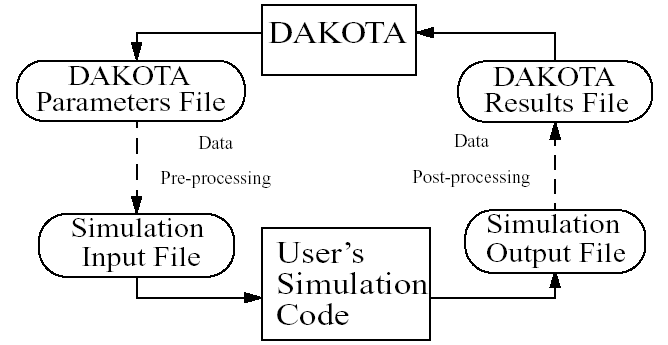
\includegraphics[height=32mm]{images/blackbox.png}
  \end{figure}
  \begin{itemize}
    \item Single, simple interface between Dakota and user's simulation code
    \item Easy to try new methods or algorithms; generally only need to change a
          few lines in the Dakota text input file
    \item Does not require deep knowledge of underlying Dakota software packages
    \item ``Black-box'' coupling: Dakota and user's simulation code
          exchange data by reading and writing short text files
    \item Closer coupling is possible for advanced users if needed
  \end{itemize}
\end{frame}

% ==============================================================================

\begin{frame}[fragile]
  \frametitle{Running Dakota with a simple input file}
  \begin{itemize}
    \item Check to make sure Dakota is in the system path
  \end{itemize}
  \begin{tiny}\begin{lstlisting}
$ dakota -v
Dakota version 6.11 released Nov 15 2019.
Repository revision c3efb375 (2019-11-07) built Apr  7 2020 10:49:05.\end{lstlisting}\end{tiny}
  \begin{itemize}
    \item Copy example input file from Dakota install directory
  \end{itemize}
  \begin{tiny}\begin{lstlisting}
$ cp -p /path/to/dakota/share/dakota/examples/users/rosen_grad_opt.in .\end{lstlisting}\end{tiny}
  \begin{itemize}
    \item Run Dakota
  \end{itemize}
  \begin{tiny}\begin{lstlisting}
$ name=rosen_grad_opt
$ dakota -i $name.in -o $name.out -w $name.rst &> $name.log\end{lstlisting}\end{tiny}
  \begin{itemize}
    \item Check for existence of Dakota output files
  \end{itemize}
  \begin{tiny}\begin{lstlisting}
$ ls -1
rosen_grad_opt.dat
rosen_grad_opt.in
rosen_grad_opt.log
rosen_grad_opt.out
rosen_grad_opt.rst\end{lstlisting}\end{tiny}
\end{frame}

% ==============================================================================

\begin{frame}
  \frametitle{Dakota output files}
  \begin{itemize}
    \item Screen output saved to a file (\lstinline{rosen_multidim.log})
    \item Output file (\lstinline{rosen_multidim.out})
    \begin{itemize}
      \item Information on the problem
      \item Information on each function evaluation
      \item Summary statistics
    \end{itemize}
    \item Tabular output file (\lstinline{rosen_multidim.dat})
    \begin{itemize}
      \item Function evaluation results in parsable format
    \end{itemize}
    \item Restart file (\lstinline{rosen_multidim.rst})
    \begin{itemize}
      \item Can use this file to restart calculation if interrupted
    \end{itemize}
  \end{itemize}
\end{frame}

% ==============================================================================

\begin{frame}
  \frametitle{Rosenbrock test problem}
  \begin{itemize}
    \item The example used here aims to find the parameters $x_1$ and $x_2$
          which minimize the Rosenbrock function:
  \end{itemize}
  \begin{equation}
    f\left(x_1,x_2\right) = 100\left(x_2-x_1^2\right)^2 + \left(1-x_1\right)^2
  \end{equation}
  \vskip -5mm
  \begin{columns}
    \column{0.5\textwidth}
    \begin{figure}
      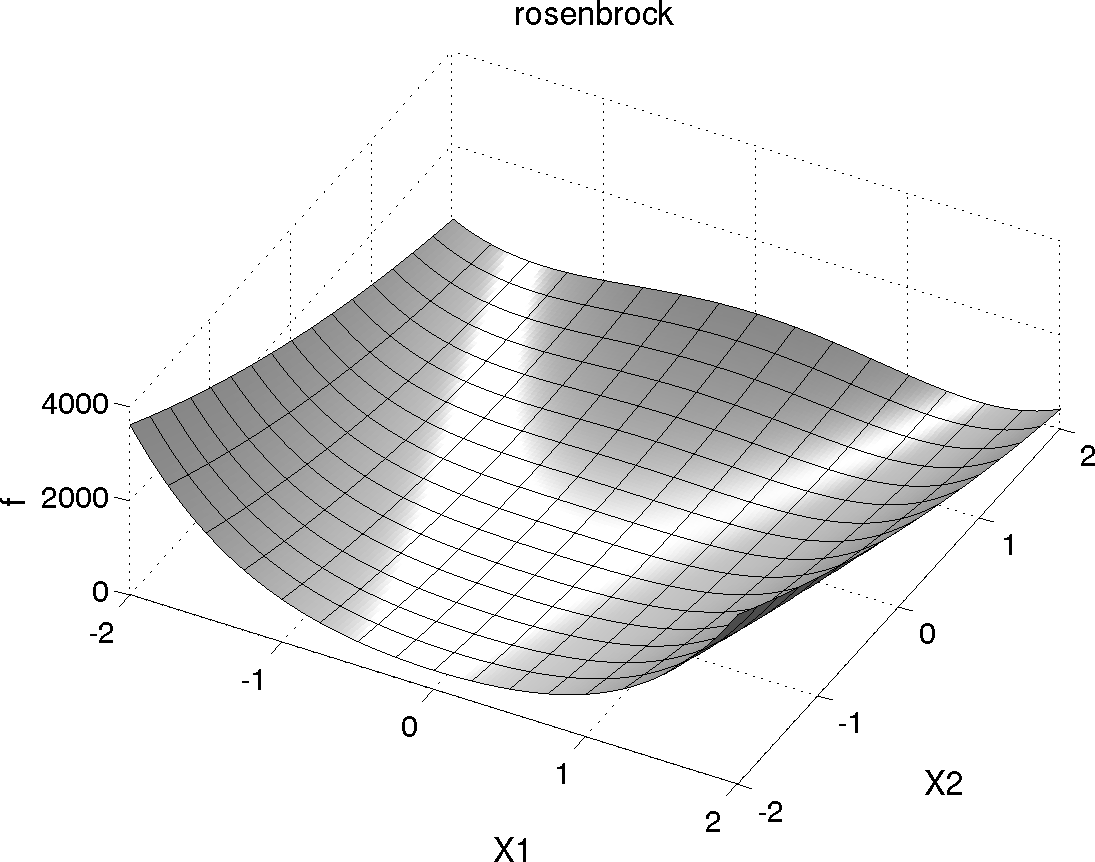
\includegraphics[height=40mm]{images/rosenbrock_3d.png}
    \end{figure}
    \column{0.5\textwidth}
    \begin{figure}
      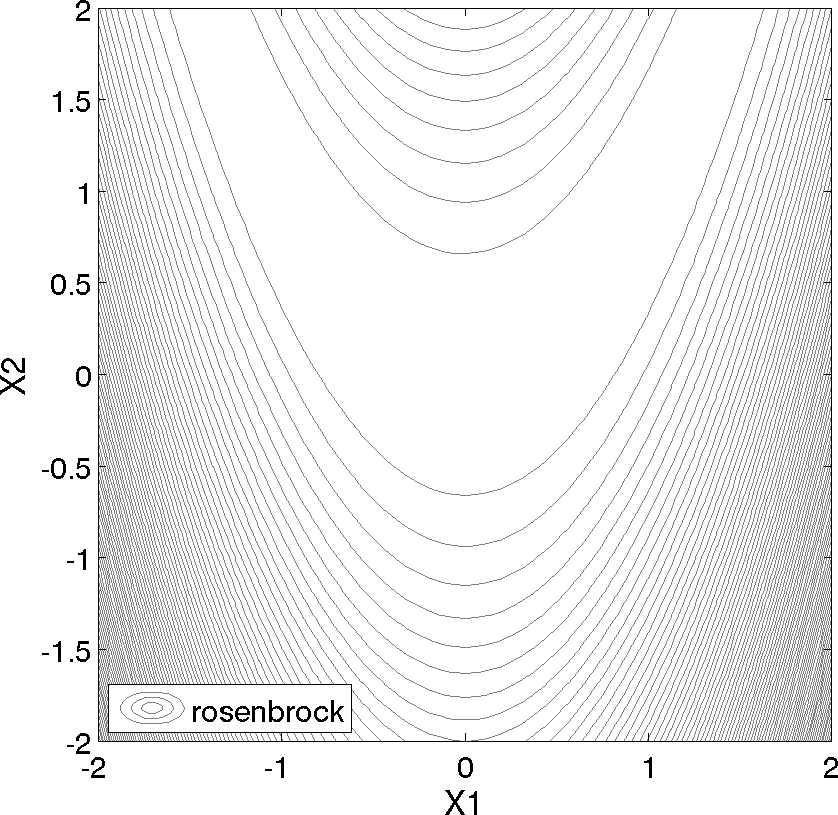
\includegraphics[height=40mm]{images/rosenbrock_contour.png}
    \end{figure}
  \end{columns}
  \begin{itemize}
    \item The problem is a gradient-based and unconstrained
    \item The problem can be solved analytically, and the unique solution lies
          at the point $\left(x_1,x_2\right) = \left(1,1\right)$, where the
          function value is 0
  \end{itemize}
\end{frame}

% ==============================================================================

\begin{frame}[fragile]
  \frametitle{Dakota output file format (1)}
  \begin{itemize}
    \item Input file repeated at top
  \end{itemize}
  \begin{tiny}\begin{lstlisting}
Dakota version 6.11 released Nov 15 2019.
Repository revision c3efb375 (2019-11-07) built Apr  7 2020 10:49:05.
Running MPI Dakota executable in serial mode.
Start time: Sun Apr 19 22:26:00 2020

-----------------------
Begin DAKOTA input file
rosen_grad_opt.in
-----------------------

***INPUT FILE SHOWN HERE***

---------------------
End DAKOTA input file
---------------------\end{lstlisting}\end{tiny}
\end{frame}

% ==============================================================================

\begin{frame}[fragile]
  \frametitle{Dakota output file format (2)}
  \begin{itemize}
    \item Information on each function evaluation, derivative estimation, etc.
          shown
  \end{itemize}
  \begin{tiny}\begin{lstlisting}
Using Dakota input file 'rosen_grad_opt.in'
Writing new restart file 'rosen_grad_opt.rst'.

>>>>> Executing environment.

>>>>> Running conmin_frcg iterator.

---------------------
Begin Evaluation    1
---------------------
Parameters for evaluation 1:
                     -1.2000000000e+00 x1
                      1.0000000000e+00 x2

Direct interface: invoking rosenbrock

Active response data for evaluation 1:
Active set vector = { 1 }
                      2.4200000000e+01 obj_fn

------------------------------------------
Begin Dakota derivative estimation routine
------------------------------------------

>>>>> map at X performed previously and results retrieved

>>>>> Dakota finite difference gradient evaluation for x[1] + h:\end{lstlisting}\end{tiny}
\end{frame}

% ==============================================================================

\begin{frame}[fragile]
  \frametitle{Dakota output file format (3)}
  \begin{tiny}\begin{lstlisting}
---------------------
Begin Evaluation    2
---------------------
Parameters for evaluation 2:
                     -1.2000120000e+00 x1
                      1.0000000000e+00 x2

Direct interface: invoking rosenbrock

Active response data for evaluation 2:
Active set vector = { 1 }
                      2.4202587296e+01 obj_fn

>>>>> Dakota finite difference gradient evaluation for x[2] + h:

---------------------
Begin Evaluation    3
---------------------
Parameters for evaluation 3:
                     -1.2000000000e+00 x1
                      1.0000100000e+00 x2

Direct interface: invoking rosenbrock

Active response data for evaluation 3:
Active set vector = { 1 }
                      2.4199120010e+01 obj_fn

>>>>> Total response returned to iterator:

Active set vector = { 2 } Deriv vars vector = { 1 2 }
 [ -2.1560798007e+02 -8.7999000000e+01 ] obj_fn gradient\end{lstlisting}\end{tiny}
\end{frame}

% ==============================================================================

\begin{frame}[fragile]
  \frametitle{Dakota output file format (4)}
  \begin{itemize}
    \item Summary data shown at the bottom
  \end{itemize}
  \begin{tiny}\begin{lstlisting}
...

---------------------
Begin Evaluation  137
---------------------
Parameters for evaluation 137:
                      9.9401208948e-01 x1
                      9.8869321157e-01 x2

Direct interface: invoking rosenbrock

Active response data for evaluation 137:
Active set vector = { 1 }
                      7.5946452397e-05 obj_fn

<<<<< Function evaluation summary: 137 total (137 new, 0 duplicate)
<<<<< Best parameters          =
                      9.9341884597e-01 x1
                      9.8744342609e-01 x2
<<<<< Best objective function  =
                      7.4943502239e-05
<<<<< Best data captured at function evaluation 136

<<<<< Iterator conmin_frcg completed.
<<<<< Environment execution completed.
DAKOTA execution time in seconds:
  Total CPU        =          0 [parent =          0, child =          0]
  Total wall clock =   0.011143\end{lstlisting}\end{tiny}
\end{frame}

% ==============================================================================

\begin{frame}[fragile]
  \frametitle{Dakota tabular output file format}
  \begin{itemize}
    \item Function evaluation results in parsable format
  \end{itemize}
  \begin{tiny}\begin{lstlisting}
%eval_id interface             x1             x2         obj_fn
1            NO_ID           -1.2              1           24.2
2            NO_ID   -1.190378659    1.003926888    21.86081004
3            NO_ID   -1.151893297    1.019634439    14.06928675
4            NO_ID   -1.027899292    1.070241789    4.131048308
5            NO_ID   -1.107874463    0.927134653    13.45821149
6            NO_ID   -1.029995089    1.066491582    4.124017963
7            NO_ID   -1.030081177    1.066337535    4.124007196
8            NO_ID  -0.9934415994    0.993092869    3.977612177
9            NO_ID  -0.8468832877   0.7001142034    3.440208959
10           NO_ID  -0.6352910806   0.2771289646    4.273536585
11           NO_ID  -0.8200039089   0.7097994601    3.452238244
12           NO_ID  -0.8339821922    0.704762764    3.372021914

...

71           NO_ID   0.9594716956   0.9244138797 0.003107859816
72           NO_ID    1.000884983   0.9989868078 0.0007758166495
73           NO_ID   0.9889662676   0.9775247703 0.0001497811442
74           NO_ID   0.9809287789   0.9819336547   0.0392215249
75           NO_ID   0.9887705737   0.9776321162 0.000126223435
76           NO_ID   0.9887766559   0.9776287799 0.0001262184309
77           NO_ID   0.9810392432    1.018933628   0.3195351433
78           NO_ID   0.9886992817   0.9780418284 0.0001542863079
79           NO_ID   0.9887719616   0.9776538396 0.000126094937
80           NO_ID    0.998581376   0.9983193227 0.0001353129642
81           NO_ID    0.993418846   0.9874434261 7.494350224e-05
82           NO_ID   0.9940120895   0.9886932116 7.59464524e-05\end{lstlisting}\end{tiny}
\end{frame}

% ==============================================================================

\begin{frame}
  \frametitle{Dakota input file format}
  \begin{columns}
    \column{0.35\textwidth}
    \newline\newline\newline
    Six specification blocks
    \begin{itemize}
      \item Environment
      \item Method
      \item Model
      \item Variables
      \item Interface
      \item Responses
    \end{itemize}
    \column{0.65\textwidth}
    \begin{figure}
      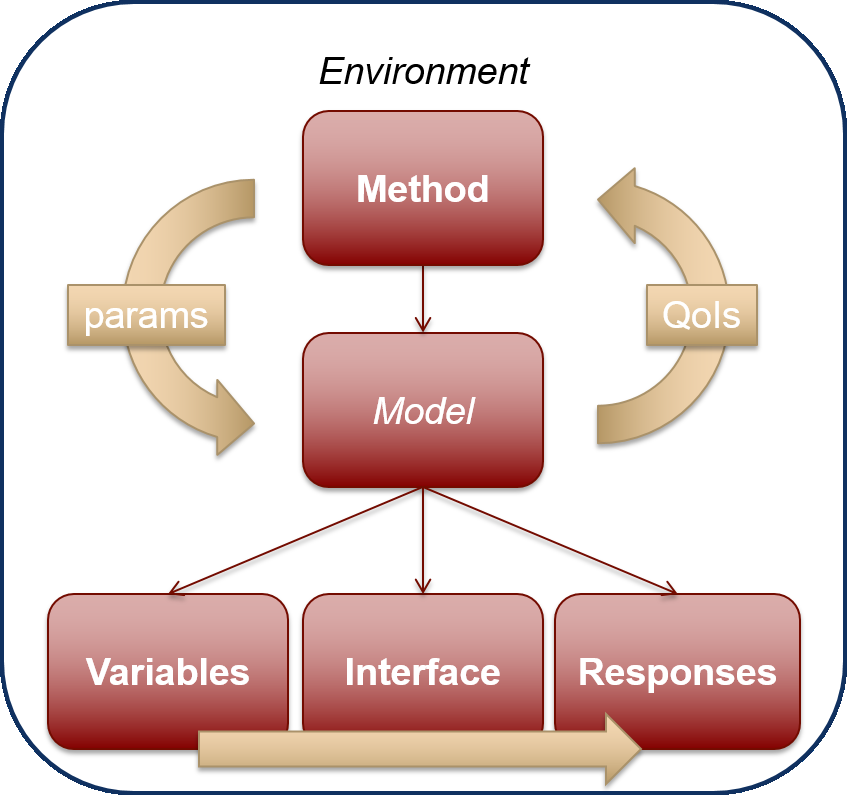
\includegraphics[width=70mm]{images/input_6_blocks.png}
    \end{figure}
  \end{columns}
\end{frame}

% ==============================================================================

\begin{frame}[fragile]
  \frametitle{Dakota input file: environment block}
  \begin{small}\begin{lstlisting}
environment
  tabular_data
    tabular_data_file = 'rosen_grad_opt.dat'\end{lstlisting}\end{small}
  \begin{itemize}
    \item Specify general settings for tabular data and graphical output
  \end{itemize}
\end{frame}

% ==============================================================================

\begin{frame}[fragile]
  \frametitle{Dakota input file: method block}
  \begin{small}\begin{lstlisting}
method
  conmin_frcg
    convergence_tolerance = 1e-4
    max_iterations = 100\end{lstlisting}\end{small}
  \begin{itemize}
    \item Specify which methods to employ and associated method options
    \item The \lstinline{conmin_frcg} option tells Dakota to employ the
          conjugate gradient optimization method located within the CONMIN
          library
    \item \lstinline{convergence_tolerance} is a relative convergence tolerance
          for the objective function; if the change in the objective function
          between successive iterations divided by the previous objective
          function is less than the specified number, then the convergence
          criterion is satisfied
    \item \lstinline{max_iterations} specifies the maximum number of iterations
  \end{itemize}
\end{frame}

% ==============================================================================

\begin{frame}[fragile]
  \frametitle{Dakota input file: model block}
  \begin{small}\begin{lstlisting}
model
  single\end{lstlisting}\end{small}
  \begin{itemize}
    \item Specify the model that Dakota will use
    \item Model provides logic for determining how variables are mapped through
          an interface into a set of responses when needed by an iterative
          method
    \item \lstinline{single} means a single set of variables, interfaces, and
          responses are specified (this is default)
    \item This block contains more information when performing advanced studies
          like surrogate-based analysis or optimization under uncertainty
  \end{itemize}
\end{frame}

% ==============================================================================

\begin{frame}[fragile]
  \frametitle{Dakota input file: variables block}
  \begin{small}\begin{lstlisting}
variables
  continuous_design = 2
    initial_point    -1.2      1.0
    lower_bounds     -2.0     -2.0
    upper_bounds      2.0      2.0
    descriptors       'x1'     "x2"\end{lstlisting}\end{small}
  \begin{footnotesize}\begin{itemize}
    \item Specify the number, type, and characteristics of parameters that will
          be varied by Dakota
    \item ``Design'' variables are mainly used in optimization and calibration
    \item ``Uncertain'' variables are mainly used in UQ and sensitivity studies
    \item ``State'' variables are mainly fixed
    \item All variables can be continuous or discrete
    \item \lstinline{continuous_design = 2} means that there are 2 continuous
          design variables
    \item \lstinline{initial_point} defines the variable starting points
    \item \lstinline{lower_bounds} and \lstinline{upper_bounds} define the range
          of values the variables are allowed to take
    \item \lstinline{descriptors} are simply names for the variables
  \end{itemize}\end{footnotesize}
\end{frame}

% ==============================================================================

\begin{frame}[fragile]
  \frametitle{Dakota input file: interface block}
  \begin{small}\begin{lstlisting}
interface
  analysis_drivers = 'rosenbrock'
    direct\end{lstlisting}\end{small}
  \begin{itemize}
    \item Specify the simulation code that will be used to map variables into
          responses
    \item Specify how Dakota will pass data to and from that code
    \item \lstinline{direct} indicates a function linked directly into Dakota
    \item \lstinline{fork} or \lstinline{system} keywords can be used to execute
          external programs
    \item Data is passed between Dakota and external programs through text files
  \end{itemize}
\end{frame}

% ==============================================================================

\begin{frame}[fragile]
  \frametitle{Dakota input file: responses block}
  \vskip -2mm
  \begin{small}\begin{lstlisting}
responses
  objective_functions = 1
# analytic_gradients
  numerical_gradients
    method_source dakota
    interval_type forward
    fd_step_size = 1.e-5
  no_hessians\end{lstlisting}\end{small}
  \begin{footnotesize}\begin{itemize}
    \item Specify the types of data that the interface will return to Dakota
    \item \lstinline{objective_functions} are used in optimization
    \item \lstinline{calibration_terms} are used in calibration
    \item \lstinline{response_functions} are used in sensitivity analysis and UQ
    \item The \lstinline{analytic_gradients} option uses Dakota's built-in
          gradient evaluation (the \lstinline{#} symbol means this line is
          commented out)
    \item The \lstinline{numerical_gradients} option tells Dakota to use the
          finite difference method to calculate gradients for the optimization
          algorithm
    \item The \lstinline{no_hessians} option tells Dakota that no second-order
          partial derivatives are used
  \end{itemize}\end{footnotesize}
\end{frame}

% ==============================================================================

\begin{frame}
  \frametitle{Rosenbrock optimization results}
  \begin{figure}
    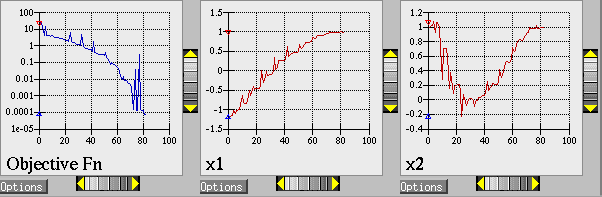
\includegraphics[width=96mm]{images/rosenbrock_values.png}
  \end{figure}
  \vskip -5mm
  \begin{columns}
    \column{0.4\textwidth}
    \begin{figure}
      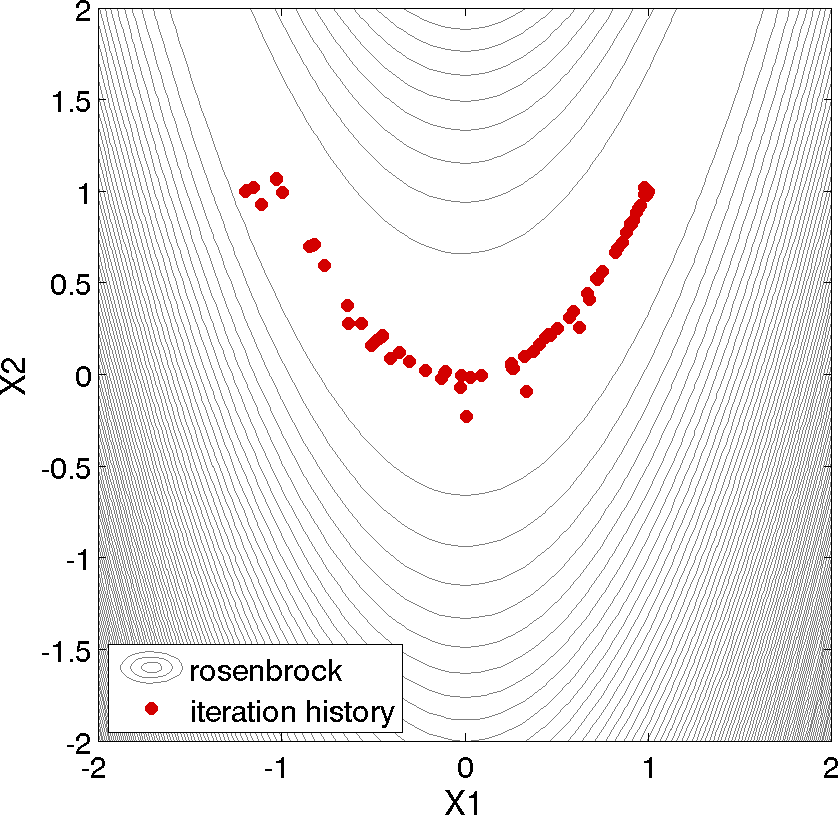
\includegraphics[height=40mm]{images/rosenbrock_contour_points.png}
    \end{figure}
    \column{0.6\textwidth}
    \begin{itemize}
      \item Above: Objective function and input parameter values for each
            iteration
      \item Left: Design points on the Rosenbrock contour plot
    \end{itemize}
  \end{columns}
\end{frame}

% ==============================================================================

\end{document}
